
Once the linear system has been built, we must solve it. 
The simplest approach is to use 
spsolve\footnote{\url{https://docs.scipy.org/doc/scipy/reference/generated/scipy.sparse.linalg.spsolve.html#scipy.sparse.linalg.spsolve}}.

\begin{lstlisting}       
sol=sps.linalg.spsolve(sparse_matrix,rhs)
\end{lstlisting}       

Another possibility is available to us: (L)GMRES\footnote{\url{https://docs.scipy.org/doc/scipy/reference/sparse.linalg.html#module-scipy.sparse.linalg}}.

\begin{lstlisting}       
sol = scipy.sparse.linalg.gmres(sparse_matrix, rhs, restart=2000,tol=1e-8)[0]
sol = scipy.sparse.linalg.lgmres(sparse_matrix, rhs,atol=1e-16,tol=1e-5)[0]
\end{lstlisting}       

Note that these solvers tend to use all resources, as shown here on my laptop with 8 cores:
\begin{center}
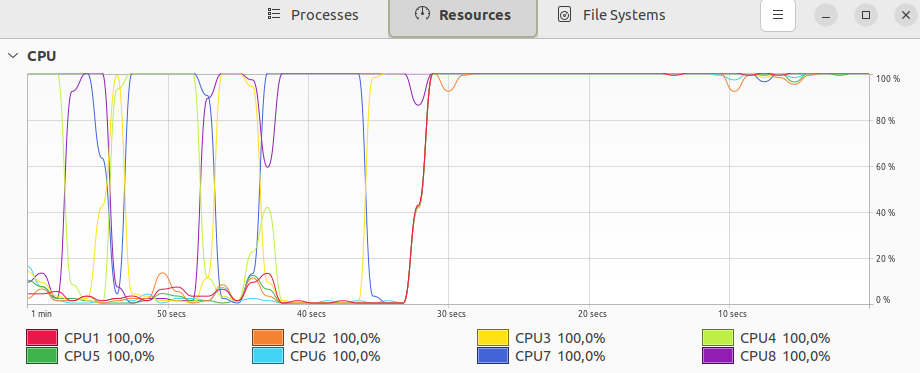
\includegraphics[width=10cm]{RESULTS/timings/resources}
\end{center}

GMRES\footnote{See the excellent blog post on GMRES at \url{https://www.rikvoorhaar.com/gmres/}} 
and LGMRES are Krylov subspace solvers. They require a (relative) tolerance
which determines the accuracy of the solution. 
Interestingly LGRMRES does not require a restart length parameter.

Note that a preconditioner could and should be supplied to the (L)GMRES 
algorithms for optimal performance \cite{krhb12}.
